%\documentclass[tikz,convert={density=800,outext=.jpg},border=5pt]{standalone}
\documentclass[tikz, border=5pt]{standalone}

\usepackage[utf8]{inputenc} % utf8 encoding
%\usepackage[english]{babel}
%\usepackage[T1]{fontenc} % use T1 fonts
\usepackage{amsmath} % nice math symbols
     

\usepackage{tikz}
\usetikzlibrary{shapes,arrows,calc}

\begin{document}
	
	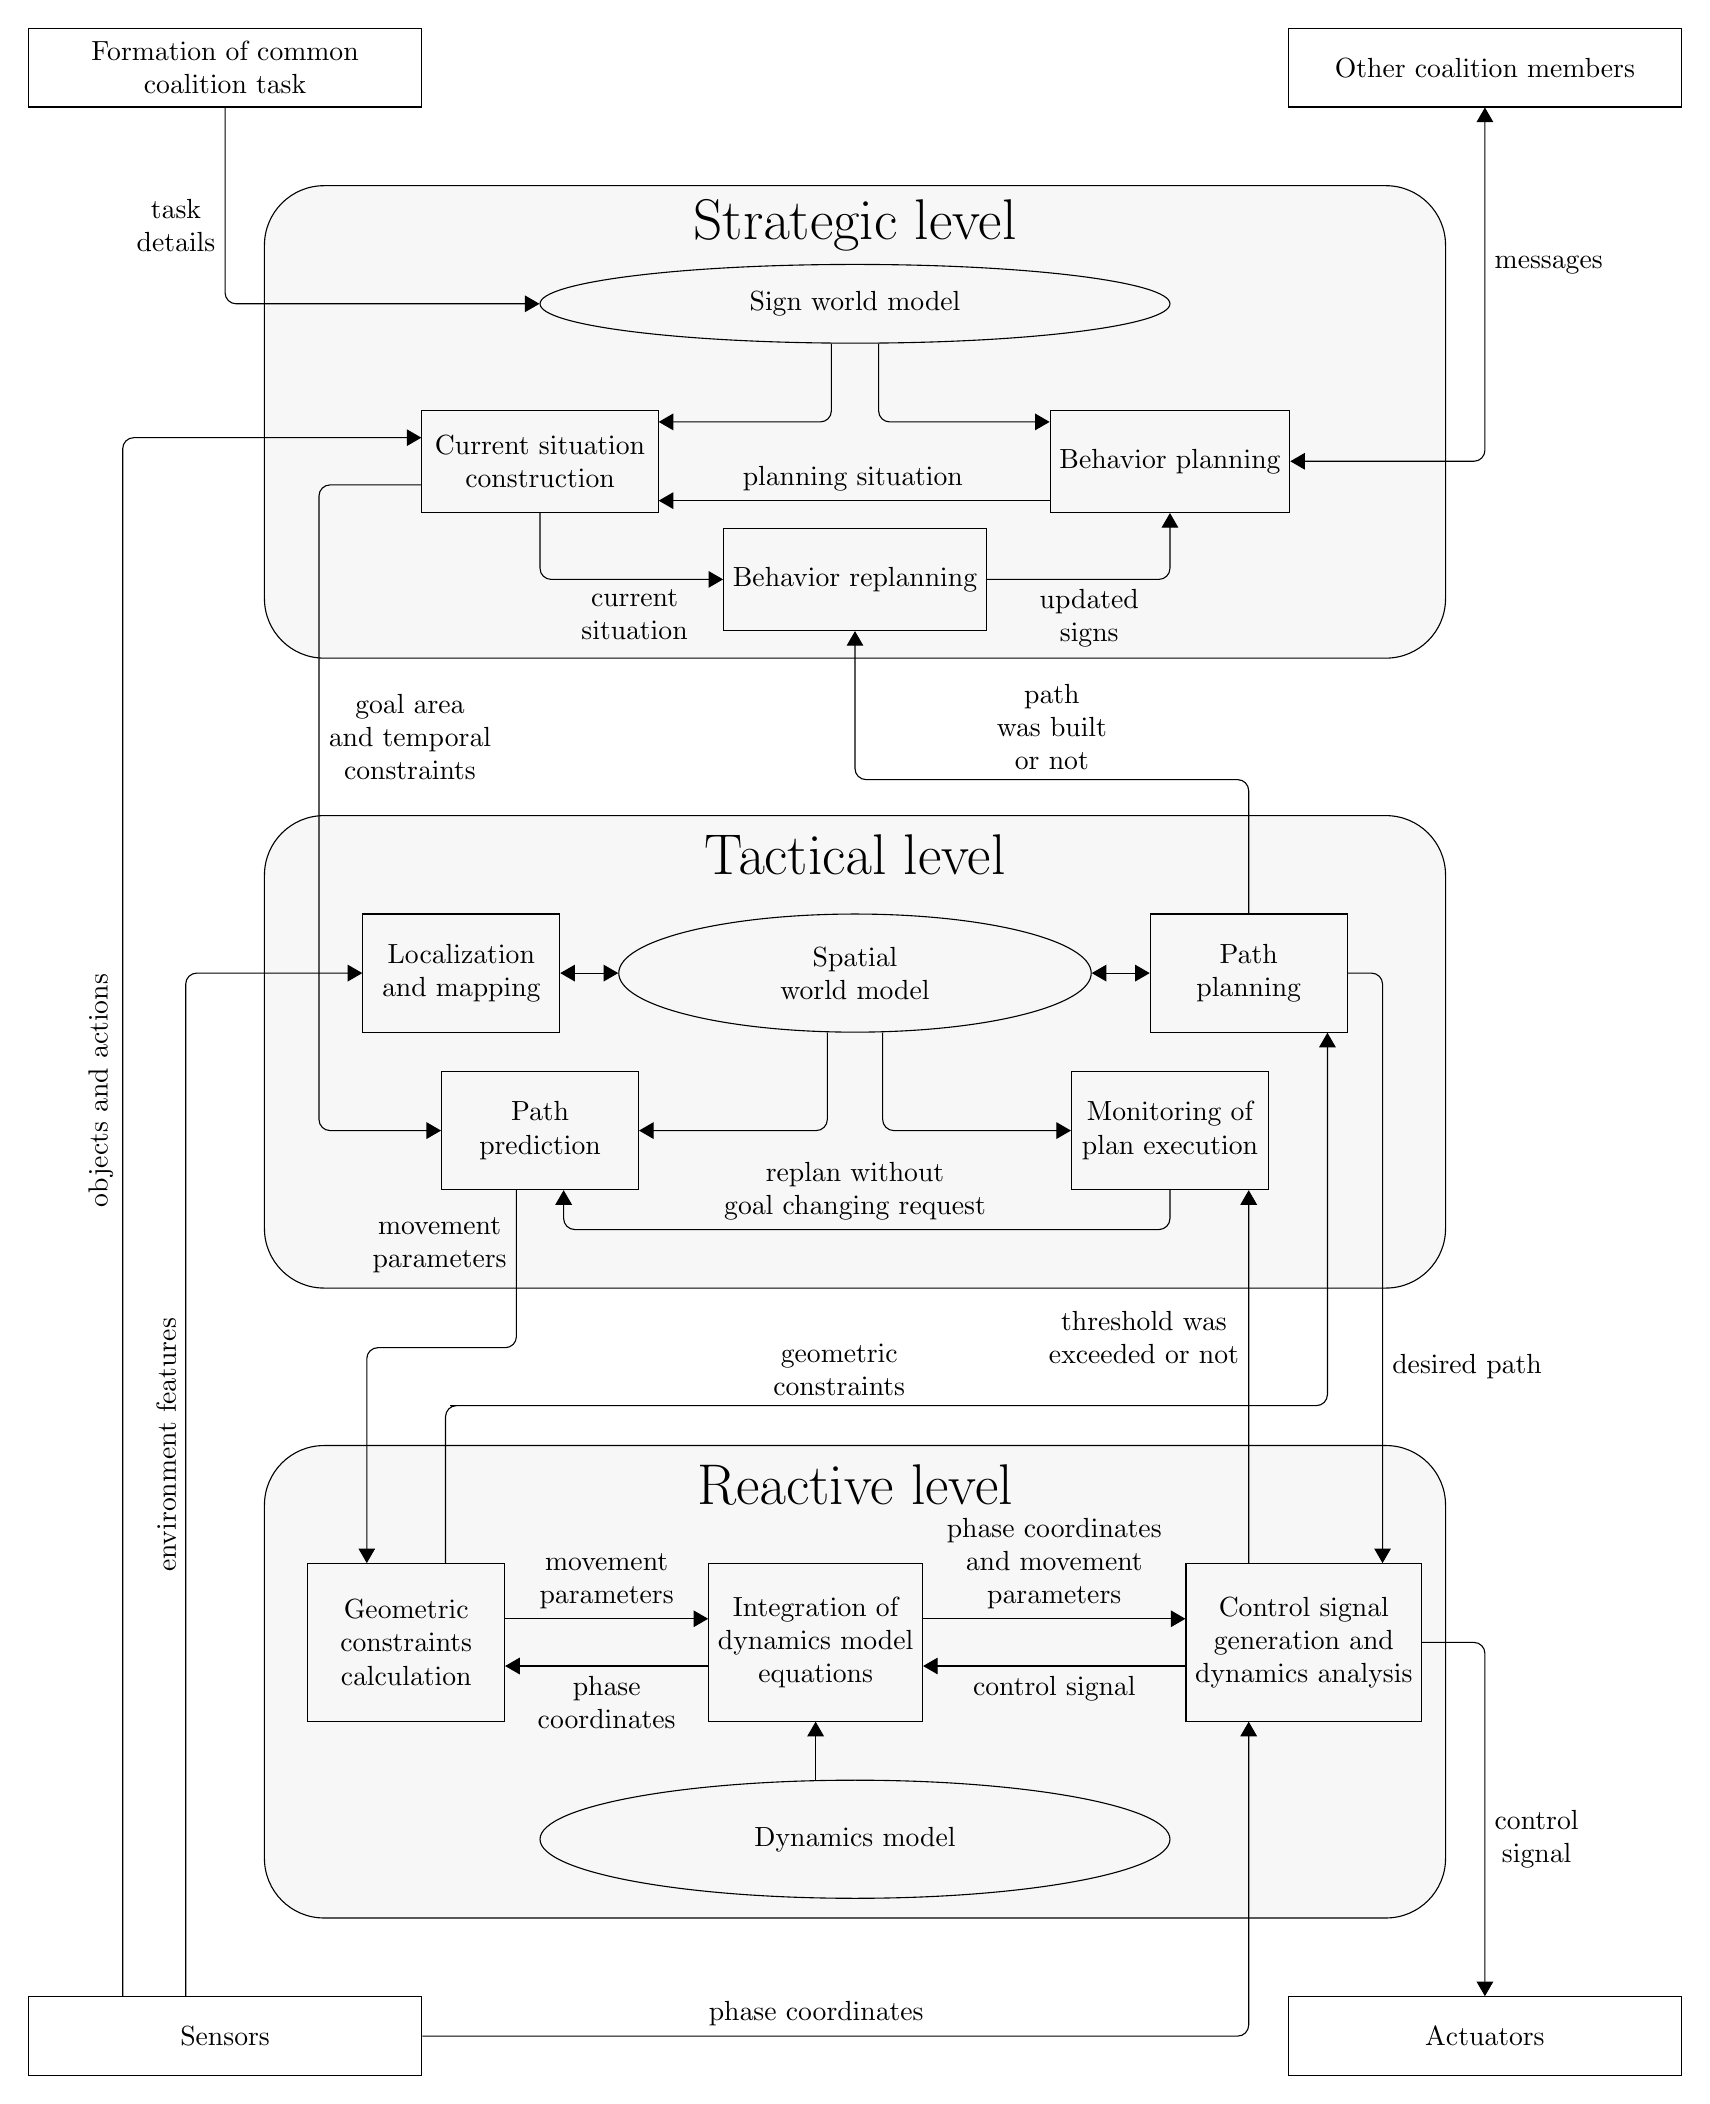
\begin{tikzpicture}[>=triangle 60]
		\tikzstyle{level_rect} = [draw, rectangle, rounded corners=5ex, minimum height = 60mm, minimum width = 150mm,fill=black!3];
		\tikzstyle{level_model} =[draw, ellipse, minimum width = 80mm, minimum height = 15mm,align = center];
		\tikzstyle{control_block} = [draw, rectangle, minimum height = 20mm, minimum width = 25mm, align=center]
		\tikzstyle{traekt_block} = [draw, rectangle, minimum height = 15mm, minimum width = 25mm, align=center]
		\tikzstyle{cons_block} = [draw, rectangle, minimum height = 13mm, minimum width = 30mm, align=center]
		\tikzstyle{misc_block} = [draw, rectangle, minimum height = 10mm, minimum width = 50mm, align=center]
		
		\node[misc_block] (messages) at (8, 20.5) {Other coalition members};
		\node[misc_block] (task) at (-8, 20.5) {Formation of common\\coalition task};
		

		\node[level_rect] (level_1) at (0, 16) {};
		\node[font=\huge] at(0, 18.5) {Strategic level};		
		\node[level_model, minimum height = 10mm] (model_1) at (0, 17.5) {Sign world model};
		\node[cons_block] (sit_decr) at (-4, 15.5) {Current situation\\construction};
		\node[cons_block] (beh_plan) at (4, 15.5) {Behavior planning};
		\node[cons_block] (replaner) at (0, 14) {Behavior replanning};
		
		\draw[->,rounded corners] ([xshift=-3mm]model_1.south) |- ([yshift=5mm]sit_decr.east);
		\draw[->,rounded corners] ([xshift=3mm]model_1.south) |- ([yshift=5mm]beh_plan.west);
		\draw[->] ([yshift=-5mm]beh_plan.west) node[align = center, xshift = -25mm, above] {planning situation}-- ([yshift=-5mm]sit_decr.east);
		
		\draw[<->,rounded corners] (messages.south) node[align = center, yshift = -20mm, right] {messages}|- (beh_plan.east);
		\draw[->,rounded corners] (task.south) node[align = center, yshift = -15mm, left] {task\\details}|- (model_1.west);
		\draw[->, rounded corners] (replaner.east) node[align = center, xshift = 13mm, below] {updated\\signs}-| (beh_plan.south);
		\draw[->, rounded corners] (sit_decr.south) |- node[align = center, xshift = 12mm, below] {current\\situation} (replaner.west);
		
		

		\node[level_rect] (level_2) at (0, 8) {};
		\node[font=\huge] at(0, 10.5) {Tactical level};		
		\node[traekt_block] (slam) at (-5, 9) {Localization\\and mapping};		
		\node[traekt_block] (pred_tr) at (-4, 7) {Path\\prediction};		
		\node[traekt_block] (build_tr) at (5, 9) {Path\\planning};		
		\node[traekt_block] (monitor) at (4, 7) {Monitoring of\\plan execution};
		\node[level_model, minimum width = 60mm] (model_3) at (0, 9) {Spatial\\world model};
		
		
		\draw[->,rounded corners] ([yshift=-3mm]sit_decr.west) -| ($(sit_decr.west)+(-13mm,-35mm)$) node[align=center, right] {goal area\\and temporal\\constraints} |- (pred_tr.west);
		\draw[->,rounded corners] (build_tr.north) |- ($(build_tr.north)+(-25mm, 17mm)$) node[align=center, above] {path\\was built\\ or not} -| (replaner.south);
		\draw[<-, rounded corners] ([xshift=3mm]pred_tr.south) |- ($(pred_tr.south)+(40mm,-5mm)$) node[align = center, above] {replan without\\goal changing request} -| (monitor.south);
		\draw[->, rounded corners] ([xshift=10]model_3.south) |- (monitor.west);
		\draw[<->, rounded corners] (model_3.east) -- (build_tr.west);
		\draw[<->, rounded corners] (model_3.west) -- (slam.east);
		\draw[->, rounded corners] ([xshift=-10]model_3.south) |- (pred_tr.east);


		\node[level_rect] (level_3) at (0, 0) {};
		\node[font=\huge] at(0, 2.5) {Reactive level};		
		\node[control_block] (geom_3) at (-5.7, 0.5) {Geometric\\constraints\\calculation};
		\node[control_block] (integr_3) at (-0.5, 0.5) {Integration of\\dynamics model\\equations};
		\node[control_block] (signal_3) at (5.7, 0.5) {Control signal\\generation and\\dynamics analysis};
		\node[level_model] (model_3) at (0, -2) {Dynamics model};
				
		\draw[->] ([yshift=3mm]geom_3.east) -- node[align = center, auto] {movement\\parameters} ([yshift=3mm]integr_3.west);
		\draw[<-] ([yshift=-3mm]geom_3.east) -- node[align = center, below] {phase\\coordinates} ([yshift=-3mm]integr_3.west);
		
		\draw[->] ([yshift=3mm]integr_3.east) -- node[align = center, auto] {phase coordinates\\and movement\\parameters} ([yshift=3mm]signal_3.west);
		\draw[<-] ([yshift=-3mm]integr_3.east) -- node[align = center, below] {control signal} ([yshift=-3mm]signal_3.west);
		
		\draw[<-] (integr_3.south) -- ([xshift=-5mm]model_3.north);
		
		\draw[->,rounded corners] ([xshift=-3mm]pred_tr.south) node[align=center,yshift=-7mm,left] {movement\\parameters}|- ($(pred_tr.south)+(-7mm,-20mm)$) -| ([xshift=-5mm]geom_3.north);
		\draw[->,rounded corners] ([xshift=5mm]geom_3.north) |- node[align=center, xshift = 50mm, auto] {geometric\\constraints} ($(geom_3.north)+(7mm,20mm)$) -| ([xshift=10mm]build_tr.south);
		\draw[->,rounded corners] (build_tr.east) -| node[align=center,yshift=-50mm,right] {desired path} ([xshift=10mm]signal_3.north);
		\draw[->,rounded corners] ([xshift=-7mm]signal_3.north) -- node[align=center, yshift = 5mm, left] {threshold was\\exceeded or not} ([xshift=10mm]monitor.south);
	
		\node[misc_block] (control_meh) at (8, -4.5) {Actuators};
		\node[misc_block] (sensors) at (-8, -4.5) {Sensors};
		
		\draw[->,rounded corners] (signal_3.east) -| (control_meh.north) node[align=center, yshift = 20mm, right] {control\\signal};
		\draw[->,rounded corners] (sensors.east) node[align = center, xshift = 50mm, above] {phase coordinates} -| ([xshift=-7mm]signal_3.south);
		\draw[->,rounded corners] ([xshift=-13mm]sensors.north) node[yshift = 115mm, rotate=90, above] {objects and actions} |- ([yshift=3mm]sit_decr.west);
		\draw[->,rounded corners] ([xshift=-5mm]sensors.north) node[yshift = 70mm, rotate=90, above] {environment features} |- (slam.west);
	\end{tikzpicture}

\end{document}